\documentclass{beamer}
\usetheme{metropolis}
\usepackage{graphicx}
\usepackage{diagbox}
\usepackage{tcolorbox}
\title{Computer Logic and Digital Circuit Design (PHYS306/COSC330): Unit 3}
\author{Jordan Hanson}
\institute{Whittier College Department of Physics and Astronomy}

\begin{document}
\maketitle

\section{Summary}

\begin{frame}{Unit 3 Summary}
\alert{Reading: chapter 7} \\
We now know how to generate and process digital data. We can do algebra, compare numbers, encode, decode, and multiplex.  \textit{How does memory work?  How is information held in digital systems?}
\begin{enumerate}
\item S-R latches
\begin{itemize}
\item Basic latch, de-bounce
\item Gated latch
\item D-latch
\end{itemize}
\item Flip-flops
\end{enumerate}
\end{frame}

\section{S-R Latches}

\begin{frame}{S-R Latches}
\begin{figure}
\centering
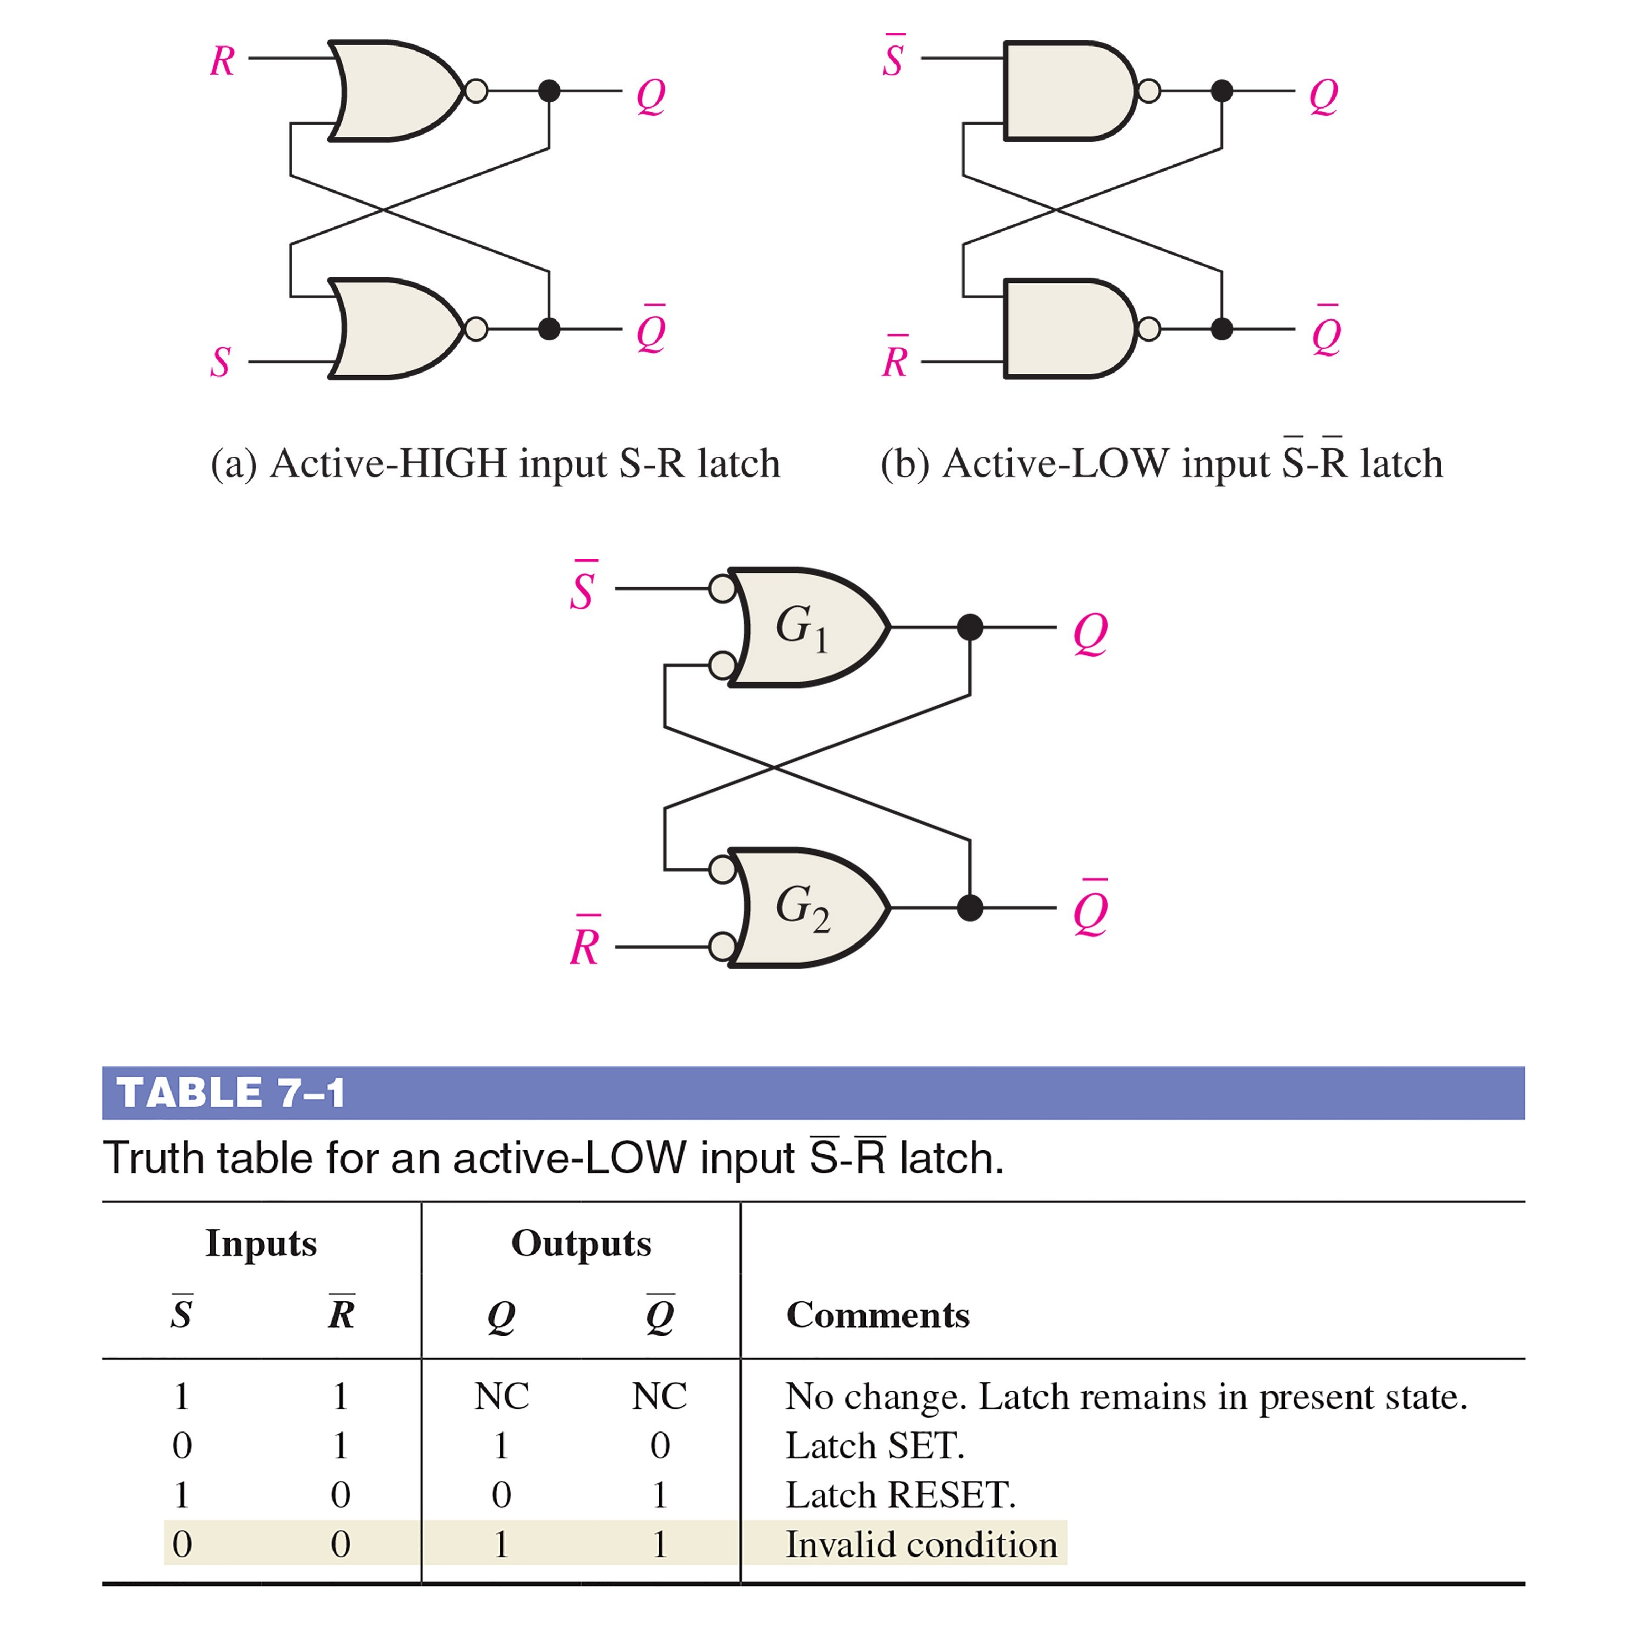
\includegraphics[width=0.55\textwidth]{figures/SR1.pdf}
\caption{\label{fig:sr1} An S-R latch is a \textit{multivibrator} that holds its state when SET, or RESET.}
\end{figure}
\end{frame}

\begin{frame}{S-R Latches}
\begin{figure}
\centering
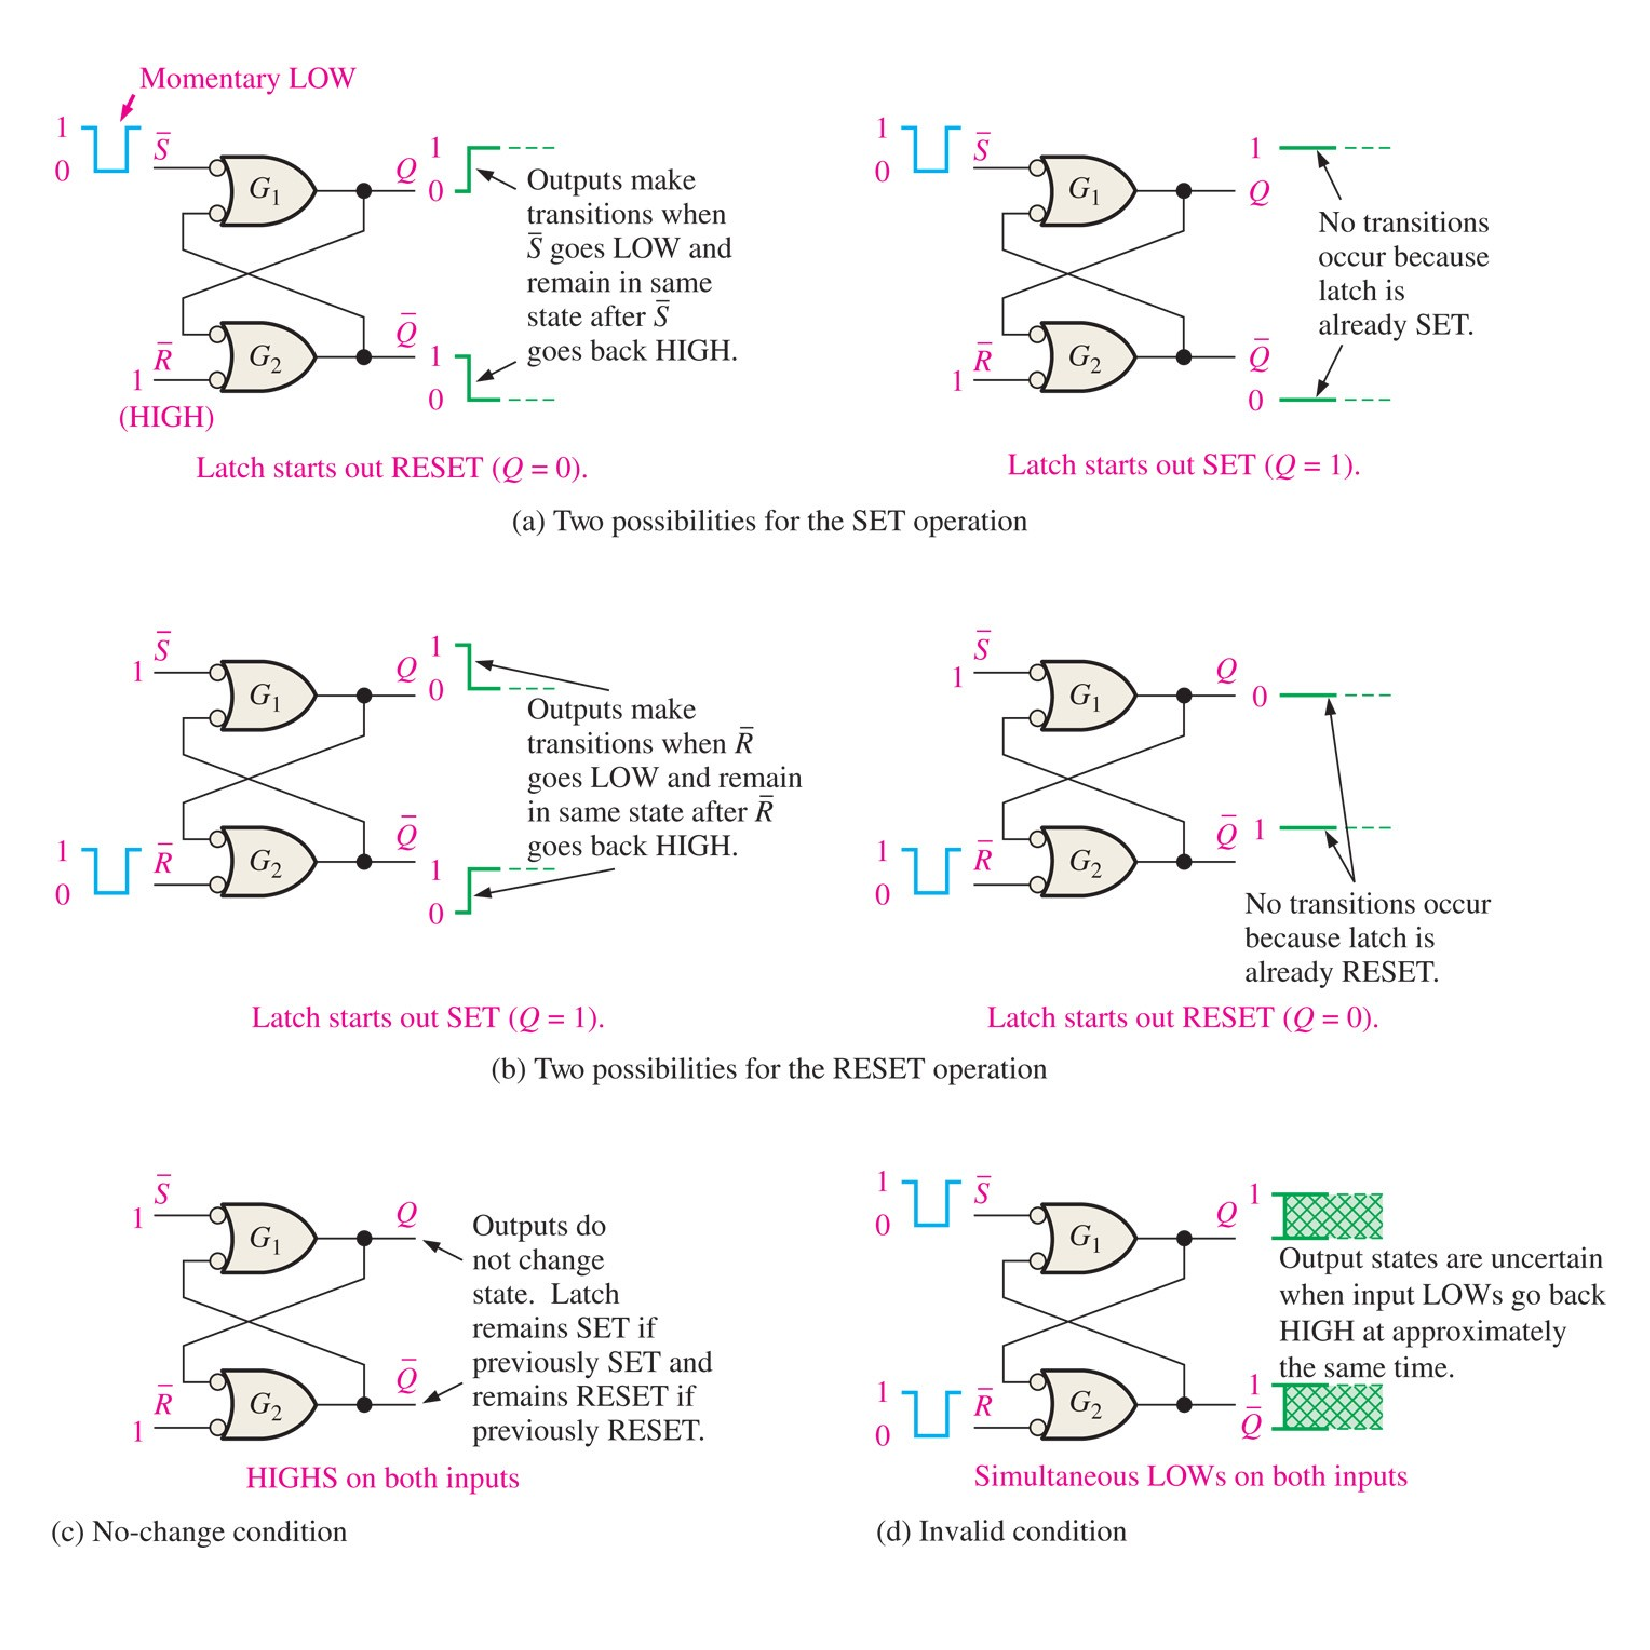
\includegraphics[width=0.55\textwidth]{figures/SR2.pdf}
\caption{\label{fig:sr2} Summary of potential states of a basic S-R latch.}
\end{figure}
\end{frame}

\begin{frame}{S-R Latches}
\begin{figure}
\centering
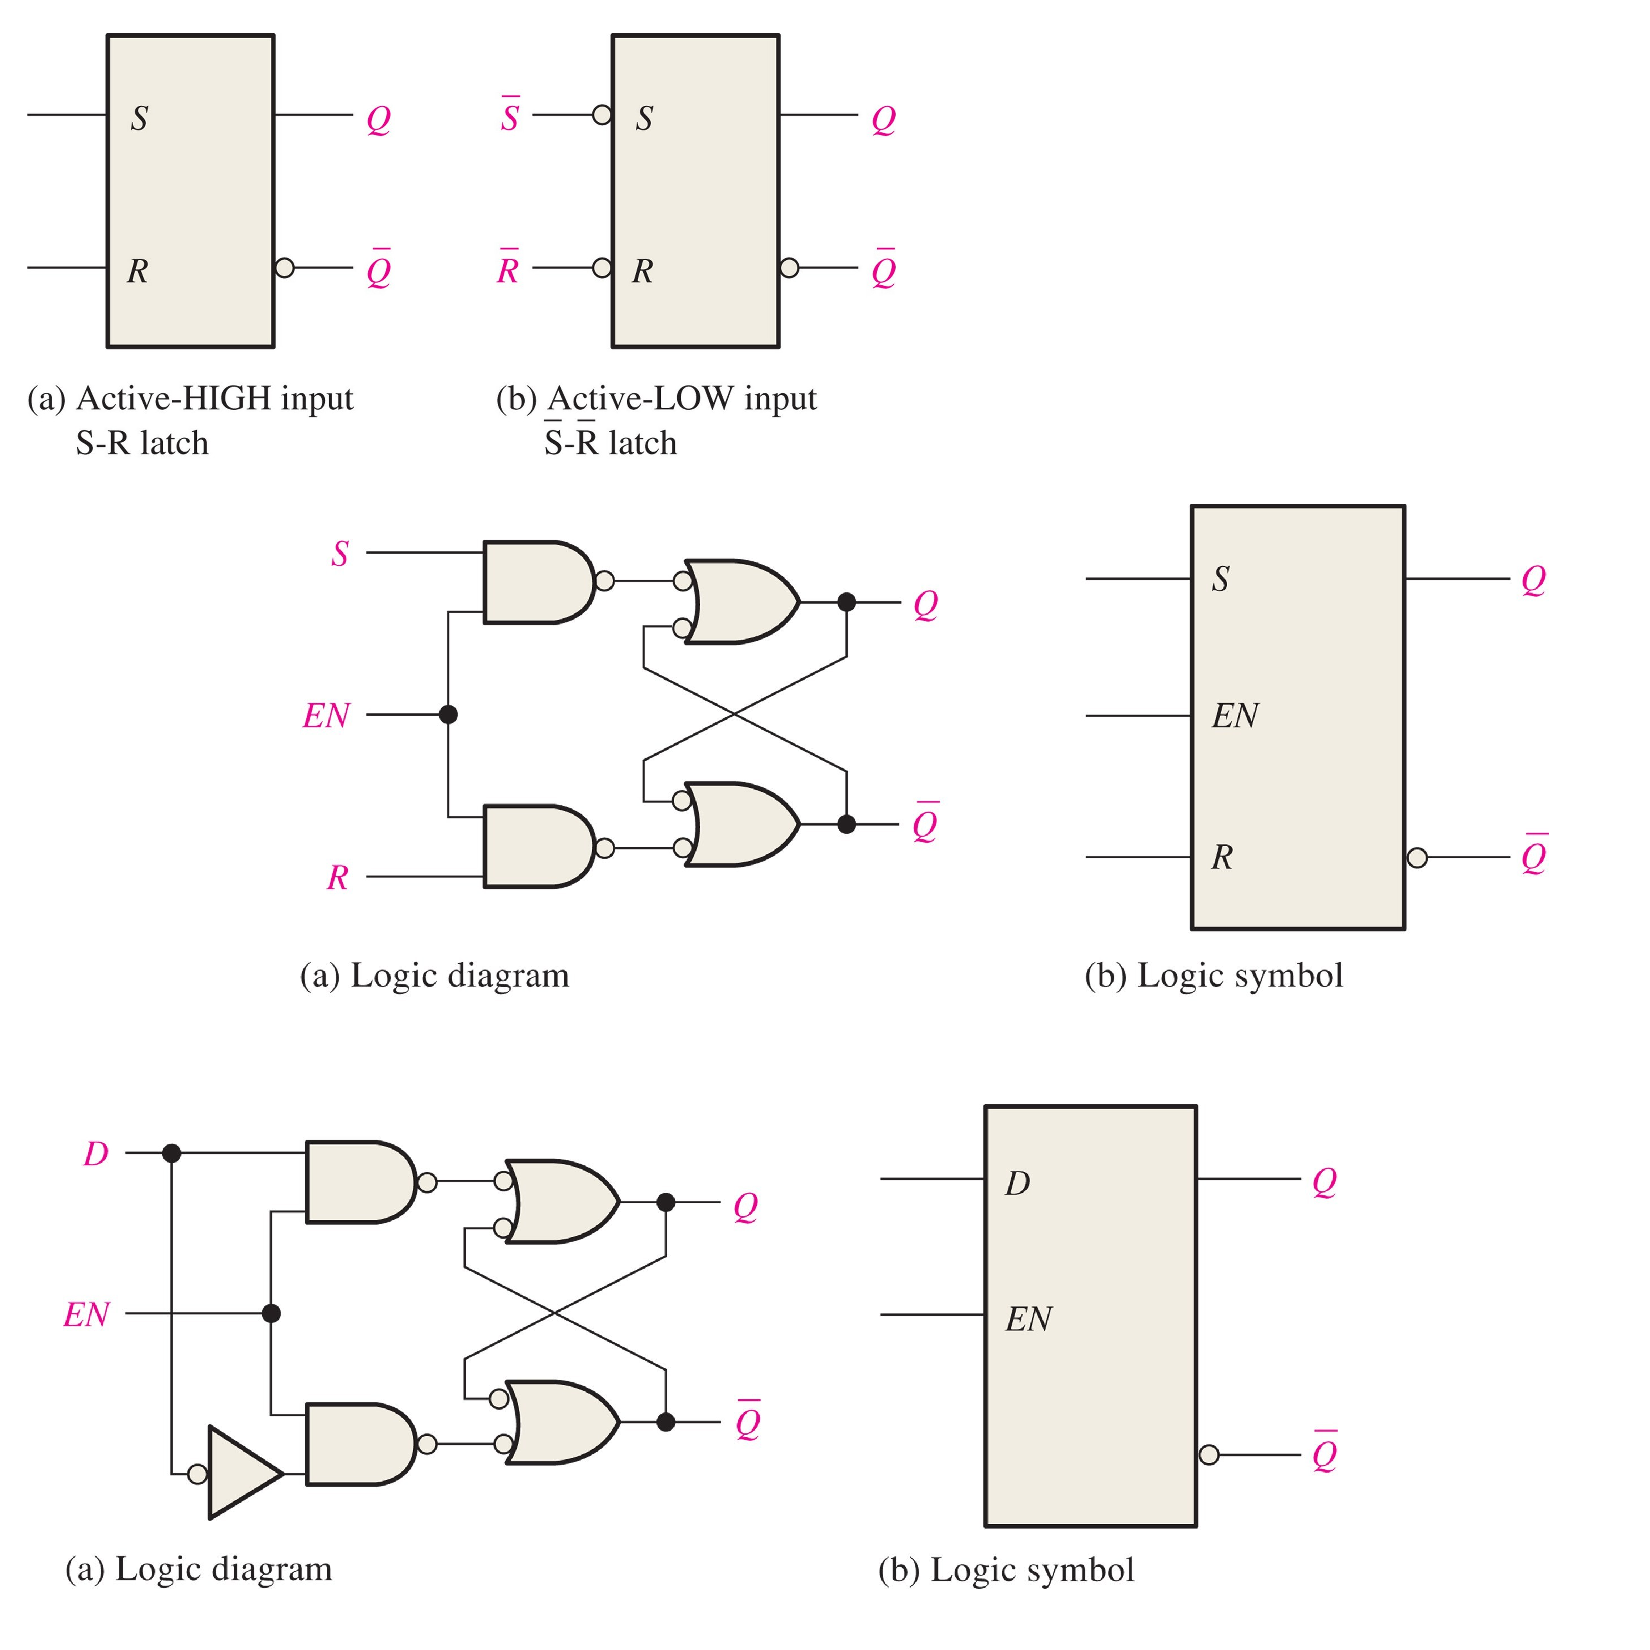
\includegraphics[width=0.55\textwidth]{figures/SR3.pdf}
\caption{\label{fig:sr3} The basic, gate-enabled, and D-latch systems.  For the latter two, both the gate and symbol are shown.}
\end{figure}
\end{frame}

\begin{frame}{S-R Latches}
\begin{figure}
\centering
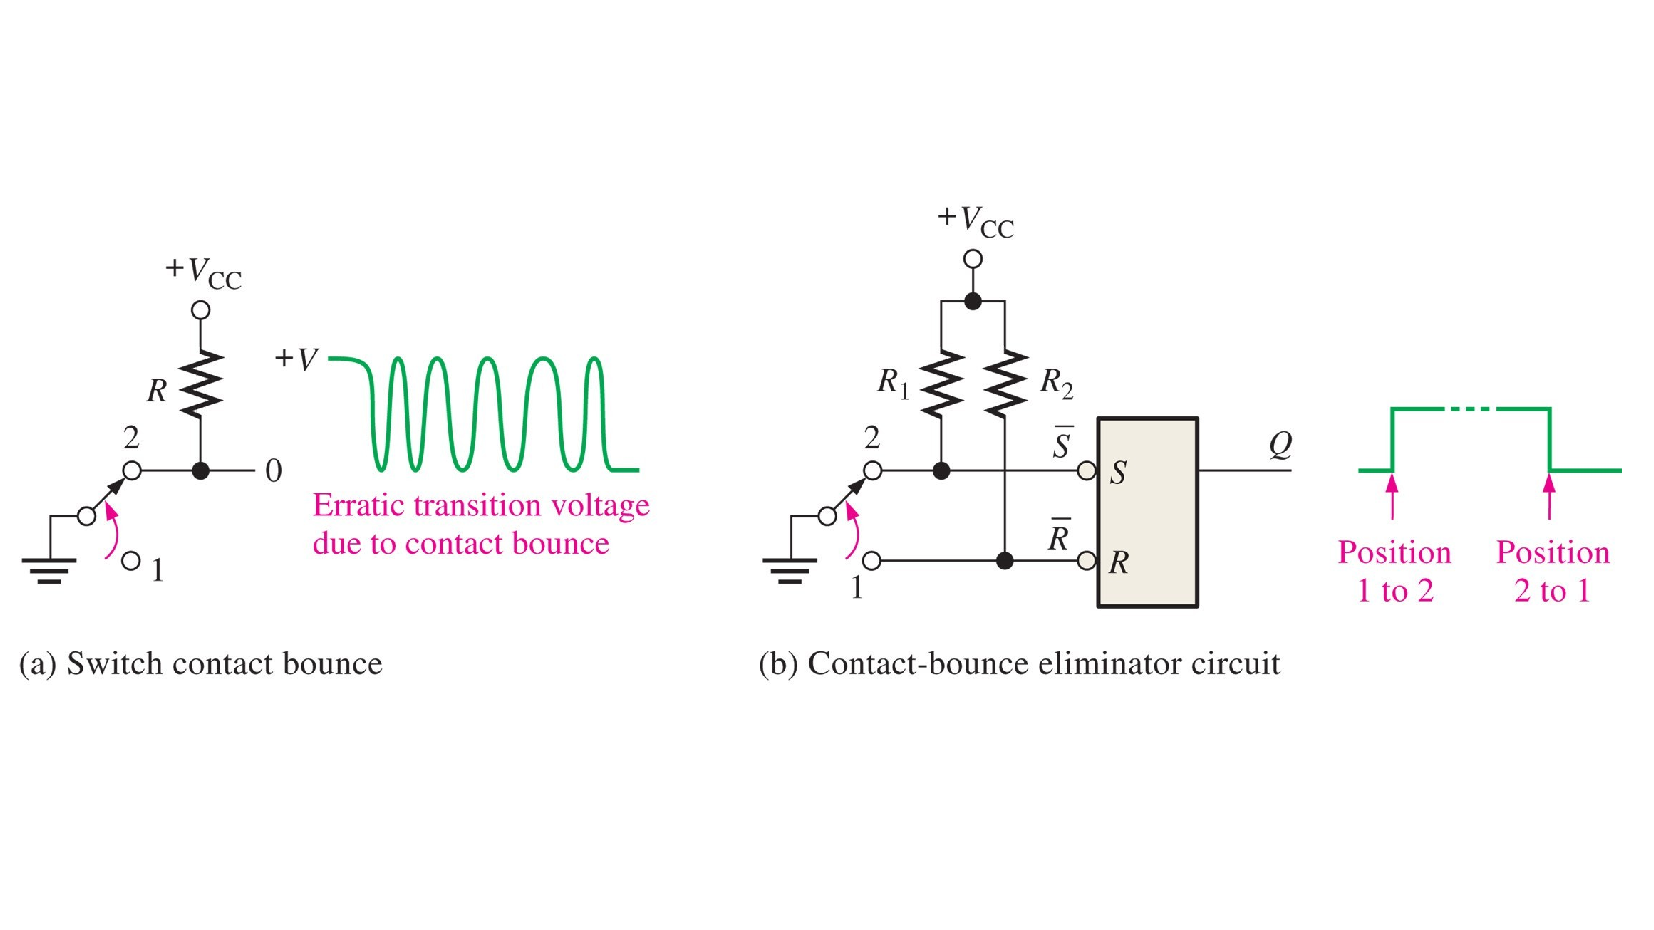
\includegraphics[width=0.85\textwidth]{figures/SR4.pdf}
\caption{\label{fig:sr4} De-bouncing is important any time a mechanical switch is meant to interact with digital logic.}
\end{figure}
\end{frame}

\section{Conclusion}

\begin{frame}{Unit 3 Summary}
\begin{enumerate}
\item things.
\end{enumerate}
\end{frame}


\end{document}
